\documentclass[aspectratio=169,10pt]{beamer}
\usetheme{Madrid}
\usecolortheme{seahorse}
\usefonttheme{professionalfonts}

\setbeamertemplate{footline}[frame number]
\setbeamertemplate{navigation symbols}{}

\graphicspath{{figures/}}

\usepackage{amsmath,amssymb,amsthm}
\usepackage{graphicx}
\usepackage{listings}
\usepackage{xcolor}
\usepackage{booktabs}

\lstset{
  basicstyle=\ttfamily\scriptsize,
  numbers=left,
  numberstyle=\tiny,
  frame=single,
  backgroundcolor=\color{gray!7},
  commentstyle=\color{green!50!black}\itshape,
  keywordstyle=\color{blue!70!black}\bfseries,
  stringstyle=\color{orange!70!black},
  breaklines=true,
  showstringspaces=false,
  language=Python
}

\newcommand{\PP}{\mathbb{P}}
\newcommand{\EE}{\mathbb{E}}
\newcommand{\RR}{\mathbb{R}}
\newcommand{\1}{\mathbbm{1}}

\title[E-Values -- Ch.16]{Hypothesis Testing with E-Values}
\subtitle{Chapter 16: E-Values and Risk Measures}
\author{Based on Ramdas \& Wang}
\date{}

\begin{document}

% ==========================================================================
\begin{frame}
\titlepage
\end{frame}

% ==========================================================================
\begin{frame}{Outline}
\tableofcontents
\end{frame}

% ==========================================================================
\section{Notation and roadmap}

\begin{frame}[allowframebreaks]{Notation you'll need}

\textbf{The big picture.} A \emph{risk measure} is just a rule that turns a random loss (or its distribution) into a single number summarizing ``how risky'' it is. This chapter (i) introduces the two most common risk measures used in finance and insurance -- Value-at-Risk and Expected Shortfall -- and a short list of ``sensible'' axioms (\emph{coherence}); (ii) shows that e-values and coherent risk measures are, mathematically, the very same object; and (iii) shows how to build e-values that test whether a risk measure exceeds some threshold.

\vspace{2mm}
\textbf{Key vocabulary (plain meaning first, formulas later):}

\begin{itemize}
\item \textbf{Risk measure $\mathcal R(X)$ or $\rho(F)$.} A number that quantifies the riskiness of a random loss $X$ (or its distribution $F$). Think of it as ``how much capital would a regulator make you set aside to cover this risk?''

\item \textbf{Value-at-Risk, $\mathrm{VaR}_\beta$.} The loss level you'd expect to be exceeded only $(1-\beta)\times 100\%$ of the time. Example: $\mathrm{VaR}_{0.95}$ is the loss level exceeded on only $5\%$ of days.

\item \textbf{Expected Shortfall, $\mathrm{ES}_\beta$.} The \emph{average} loss, given that you are already in that worst $(1-\beta)\times100\%$ of outcomes. It answers ``if things go bad, how bad on average?'', not just ``how bad at the boundary?''

\item \textbf{Coherent risk measure.} A risk measure satisfying four sensible axioms (monotonicity, cash invariance, subadditivity, positive homogeneity) -- detailed on the next slide. $\mathrm{ES}_\beta$ is coherent; $\mathrm{VaR}_\beta$ is \emph{not} (it fails subadditivity).

\framebreak

\item \textbf{Super-expectation / worst-case expectation.} $\mathcal R(X) = \sup_{\PP \in \mathcal P} \EE^{\PP}[X]$: the largest expected value of $X$ over a whole family $\mathcal P$ of candidate probability measures. This is the central bridge between risk measures and e-values in Section 16.2.

\item \textbf{E-statistic $e(x,r)$.} A recipe that converts one observed data point $x$ and a candidate risk forecast $r$ into a number $e(x,r) \ge 0$ that behaves like an e-variable whenever the true risk is $\le r$. Feeding in a whole sequence of data points builds a sequential test of ``is my risk forecast $r$ good enough?''

\item \textbf{Backtest e-statistic.} An e-statistic with real teeth: it not only stays $\le 1$ in expectation under the null ($\rho(F)\le r$), but is guaranteed to have expectation $>1$ (i.e., real power) whenever the true risk measure exceeds the forecast, $\rho(F) > r$.

\item \textbf{Monotone.} A backtest e-statistic where $r \mapsto e(x,r)$ is decreasing: reporting a \emph{larger} (more conservative) risk forecast $r$ can only make the e-statistic smaller or equal, never larger -- so there is no incentive to under-report risk.
\end{itemize}

\end{frame}

% ==========================================================================
\section{16.1 Risk measures and statistical functions}

\begin{frame}{16.1 Intuition: what problem are risk measures solving?}

\textbf{The finance story.} A bank holds a portfolio whose overnight loss is a random variable $X$ (positive $X$ = you lost money; negative $X$ = you made money). A regulator wants a single number that says ``keep at least this much capital in reserve, in case things go badly.'' That number is $\mathcal R(X)$.

\vspace{2mm}
\textbf{Two flavors of the same idea.}
\begin{itemize}
\item $\mathcal R: \mathcal X \to (-\infty,\infty]$ maps a \emph{random variable} $X$ (the loss itself) to a risk number.
\item $\rho: \mathcal M_1(\RR) \to (-\infty,\infty]$ maps a \emph{distribution} $F$ to a risk number.
\end{itemize}
These two views coincide exactly when $\mathcal R$ is \emph{law invariant}: $\mathcal R(X)=\mathcal R(Y)$ whenever $X \stackrel{\mathrm d}{=} Y$. In that case $\mathcal R$ (or $\rho$) is also called a \textbf{statistical function} -- the same idea used for the mean, variance, or median.

\vspace{2mm}
\textbf{Two everyday examples first.} Before the formal definitions: \emph{VaR at 95\%} is the loss level you'd expect to exceed only 5\% of the time (a threshold you rarely breach). \emph{ES at 95\%} is the average loss \textbf{given} that you're already in that worst 5\% (how bad is bad, on average).

\end{frame}

% ---------------------------------------------------------------------------
\begin{frame}{Definition: Value-at-Risk and Expected Shortfall}

\begin{block}{VaR: the left $\beta$-quantile}
For $\beta \in (0,1)$,
\[
\mathrm{VaR}_\beta(F) = \inf\{x \in \RR : F(x) \ge \beta\}, \qquad F \in \mathcal M_1(\RR).
\]
\emph{Symbols:} $F$ is the cdf of the loss; $\beta$ is the confidence level (e.g.\ $0.95$); $\mathrm{VaR}_\beta(F)$ is the smallest loss level $x$ such that at least a $\beta$ fraction of outcomes are $\le x$ -- equivalently, the loss is exceeded with probability at most $1-\beta$.
\end{block}

\begin{block}{ES: the average VaR beyond level $\beta$}
\[
\mathrm{ES}_\beta(F) = \frac{1}{1-\beta}\int_\beta^1 \mathrm{VaR}_\gamma(F)\, \mathrm d\gamma, \qquad F \in \mathcal M_1(\RR).
\]
\emph{Symbols:} we average the quantile function $\mathrm{VaR}_\gamma(F)$ over all confidence levels $\gamma$ from $\beta$ up to $1$, then normalize by the length $1-\beta$ of that interval. $\mathrm{ES}_\beta$ can equal $+\infty$ if $F$ has no finite mean. ES is also called Conditional VaR (CVaR) or Tail VaR (TVaR).
\end{block}

\textbf{Regulatory note.} As of 2025, $\mathrm{ES}_{0.975}$ is the Basel Committee's standard market-risk measure; $\mathrm{VaR}_\beta$ (various $\beta$) remains standard in insurance and for probability-of-default criteria.

\end{frame}

% ---------------------------------------------------------------------------
\begin{frame}{VaR and ES as optimization problems}

\begin{block}{Equations (16.1)--(16.2): the ``optimal reserve'' representation}
For $X$ with finite mean, under the reference measure $\PP_0$,
\[
\mathrm{VaR}_\beta(X) \in \operatorname*{arg\,min}_{z \in \RR} \left\{ z + \frac{1}{1-\beta}\EE^{\PP_0}[(X-z)_+] \right\},
\]
\[
\mathrm{ES}_\beta(X) = \min_{z \in \RR} \left\{ z + \frac{1}{1-\beta}\EE^{\PP_0}[(X-z)_+] \right\}.
\]
\emph{Symbols:} $z$ is a trial capital reserve; $(X-z)_+ = \max(X-z,0)$ is the shortfall beyond $z$; the objective balances holding reserve $z$ against the (scaled) expected shortfall beyond it. The minimizer $z^\star$ is $\mathrm{VaR}_\beta(X)$, and the minimal objective value is $\mathrm{ES}_\beta(X)$.
\end{block}

\textbf{Intuition.} This says: ES is literally the best achievable value of ``reserve plus scaled expected excess loss,'' and the optimal reserve to hold turns out to be exactly the VaR. This variational formula will resurface (Section 16.2) as the key link to e-values.

\end{frame}

% ---------------------------------------------------------------------------
\begin{frame}{Coherent risk measures: four sensible axioms}

\textbf{Plain-English idea.} We want risk measures that behave the way common sense says a ``good'' risk measure should. Let $\mathcal X_{\mathcal R} \subseteq \mathcal X$ be a convex cone containing all constants.

\begin{block}{Definition: coherent risk measure}
$\mathcal R: \mathcal X_{\mathcal R} \to (-\infty,\infty]$ is \textbf{coherent} if it satisfies:
\begin{itemize}
\item[(i)] \textbf{Monotonicity:} $\mathcal R(X) \le \mathcal R(Y)$ whenever $X \le Y$. \\ \emph{Real-world meaning:} a portfolio that always loses at least as much as another is at least as risky.
\item[(ii)] \textbf{Cash invariance:} $\mathcal R(X+c) = \mathcal R(X)+c$ for $c \in \RR$. \\ \emph{Real-world meaning:} adding $c$ dollars of guaranteed cash to your position reduces your required reserve by exactly $c$.
\item[(iii)] \textbf{Subadditivity:} $\mathcal R(X+Y) \le \mathcal R(X)+\mathcal R(Y)$. \\ \emph{Real-world meaning:} diversification cannot make you riskier -- merging two portfolios is never worse than holding them separately.
\item[(iv)] \textbf{Positive homogeneity:} $\mathcal R(\lambda X) = \lambda \mathcal R(X)$ for $\lambda>0$. \\ \emph{Real-world meaning:} doubling the size of a position exactly doubles its risk (no economies or diseconomies of scale).
\end{itemize}
\end{block}

\textbf{Fact.} Subadditivity + positive homogeneity together imply \emph{convexity} of $\mathcal R$.

\end{frame}

% ---------------------------------------------------------------------------
\begin{frame}{Is VaR coherent? Is ES coherent?}

\begin{block}{Result stated in the book}
For $\beta \in (0,1)$: $\mathrm{ES}_\beta : \mathcal X \to (-\infty,\infty]$ satisfies \emph{all four} axioms, so it is coherent. $\mathrm{VaR}_\beta : \mathcal X \to \RR$ satisfies all axioms \emph{except subadditivity}, so it is \emph{not} coherent.
\end{block}

\textbf{Why this matters in one sentence.} VaR can penalize diversification: it is possible to construct two positions where $\mathrm{VaR}_\beta(X+Y) > \mathrm{VaR}_\beta(X) + \mathrm{VaR}_\beta(Y)$, i.e.\ merging portfolios looks \emph{riskier} under VaR even though economically it should not be -- this is the single biggest historical criticism of VaR as a regulatory tool, and the main reason regulators moved toward ES.

\vspace{2mm}
\begin{block}{Continuity from above ($\downarrow$-continuity)}
$\mathcal R: \mathcal X_{\mathcal R} \to (-\infty,\infty]$ is $\downarrow$-continuous if $\mathcal R(X_n) \to \mathcal R(X)$ for any bounded sequence $(X_n)_{n\in\mathbb N} \downarrow X$ (pointwise decreasing convergence). This regularity condition is needed for the representation theorem in the next section.
\end{block}

\end{frame}

% ---------------------------------------------------------------------------
\begin{frame}[fragile]{Python: computing VaR and ES from simulated data}

\begin{lstlisting}
import numpy as np

def empirical_var(losses, beta):
    """VaR_beta(F) = inf{x : F(x) >= beta}, F = empirical cdf of `losses`."""
    x = np.sort(losses)
    n = len(x)
    k = int(np.ceil(beta * n))     # smallest k with k/n >= beta
    k = min(max(k, 1), n)
    return x[k - 1]                # 1-indexed k-th smallest -> index k-1

def empirical_es(losses, beta):
    """ES_beta(F) = (1/(1-beta)) * integral_beta^1 VaR_gamma(F) dgamma,
    computed exactly for the empirical (n-point) distribution."""
    x = np.sort(losses)
    n = len(x)
    # VaR_gamma is a step function, constant = x[k-1] for gamma in ((k-1)/n, k/n]
    total, k = 0.0, int(np.ceil(beta * n))
    for i in range(k, n + 1):
        lo = max(beta, (i - 1) / n)
        hi = i / n
        total += (hi - lo) * x[i - 1]
    return total / (1 - beta)

np.random.seed(1)
losses = np.random.normal(loc=0.5, scale=2.0, size=100_000)  # simulated daily losses

for beta in [0.90, 0.95, 0.975, 0.99]:
    v = empirical_var(losses, beta)
    e = empirical_es(losses, beta)
    print(f"beta={beta:5.3f}  VaR={v:6.3f}  ES={e:6.3f}  (ES >= VaR: {e >= v})")
\end{lstlisting}

\end{frame}

% ---------------------------------------------------------------------------
\begin{frame}{Figure: VaR and ES on a loss density}

\begin{center}
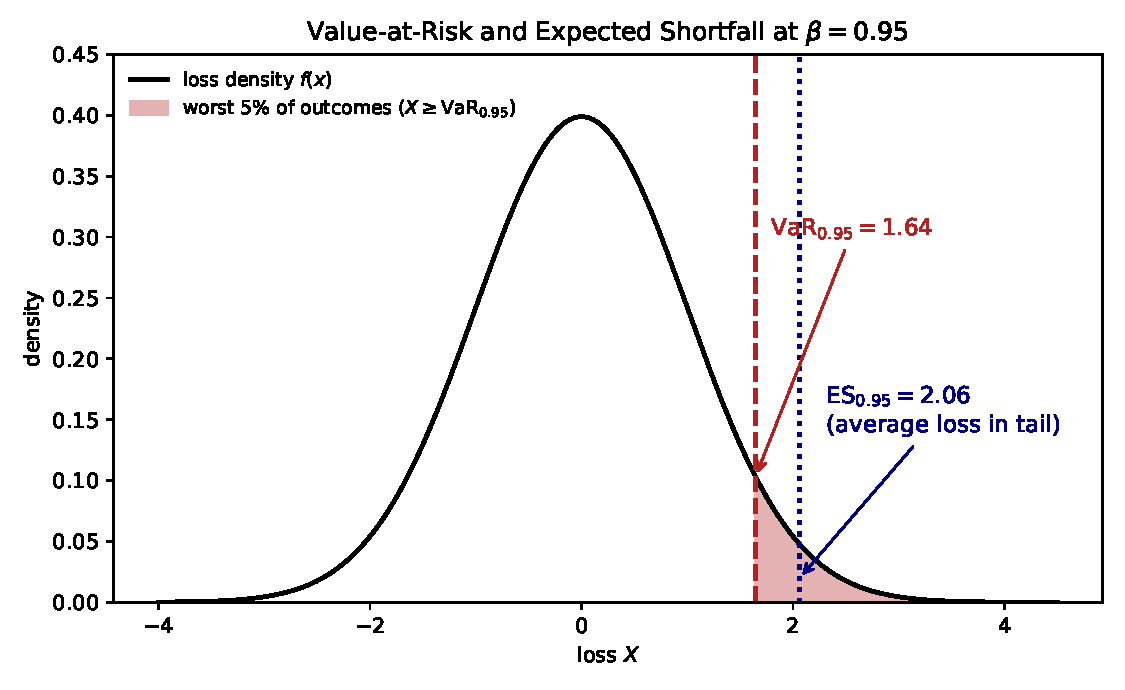
\includegraphics[width=0.72\textwidth]{fig1_var_es.pdf}
\end{center}
\vspace{-2mm}
{\footnotesize A standard-normal loss density with $\mathrm{VaR}_{0.95}$ marking the boundary of the worst $5\%$ of outcomes (shaded), and $\mathrm{ES}_{0.95}$ marking the average loss within that shaded tail. Note $\mathrm{ES}_{0.95} \ge \mathrm{VaR}_{0.95}$ always.}

\end{frame}

% ==========================================================================
\section{16.2 Connecting e-values to coherent risk measures}

\begin{frame}{16.2 Intuition: e-variables ARE a risk-measure constraint}

\textbf{The key observation.} Recall an e-variable for null hypothesis $\mathcal P$ is just a nonnegative random variable $E$ with $\EE^{\PP}[E] \le 1$ for every $\PP \in \mathcal P$. Define
\[
\mathcal R(X) = \sup_{\PP \in \mathcal P} \EE^{\PP}[X].
\]
Then ``$E$ is an e-variable'' is \emph{exactly} the constraint $\mathcal R(E) \le 1$. There is nothing more to it: \textbf{being an e-value is a risk-measure constraint}, where the risk measure $\mathcal R$ is the \emph{worst-case expectation} (a ``super-expectation'') over the null set $\mathcal P$.

\vspace{2mm}
\textbf{Why we should care.} This super-expectation $\mathcal R$ has appeared for decades in robust statistics, decision theory, finance, imprecise probability, and game-theoretic probability under different names. The point of this section: $\mathcal R$ is \emph{always} a coherent risk measure, and (with mild regularity) \emph{every} coherent risk measure arises this way. So e-values and coherent risk measures are, essentially, the same mathematical object viewed from two directions.

\end{frame}

% ---------------------------------------------------------------------------
\begin{frame}{Theorem 16.3: the representation theorem}

\begin{block}{Theorem 16.3}
Let $\mathcal X_{B+}$ be the set of all bounded nonnegative random variables. A mapping $\mathcal R: \mathcal X_{B+}\to \RR$ is a $\downarrow$-continuous coherent risk measure if and only if
\[
\mathcal R(X) = \sup_{\PP \in \mathcal P} \EE^{\PP}[X], \qquad X \in \mathcal X_{B+}
\]
for some set $\mathcal P \subseteq \mathcal M_1$.
\end{block}

\textbf{Reading it.} ``If'': any super-expectation over a family $\mathcal P$ is automatically coherent -- easy to check directly against the four axioms. ``Only if'' (the interesting direction): \emph{every} coherent, $\downarrow$-continuous risk measure, no matter how it was originally defined, secretly has this super-expectation form for some (possibly huge, possibly infinite) family $\mathcal P$ of probability measures.

\vspace{2mm}
\textbf{Proof sketch.} Extend $\mathcal R$ from $\mathcal X_{B+}$ to all bounded random variables $\mathcal X_B$ via cash invariance: $\mathcal R(X) = \mathcal R(X-t)+t$ where $t=\inf X$. Then invoke a classical representation result for coherent risk measures on $\mathcal X_B$ (Theorem 4.22 of F\"ollmer and Schied, 2016), which gives exactly the sup-of-expectations form; restrict back down to $\mathcal X_{B+}$.

\end{frame}

% ---------------------------------------------------------------------------
\begin{frame}{Corollary 16.4: e-variables are precisely a coherent constraint}

\begin{block}{Corollary 16.4}
For any null hypothesis $\mathcal P$, there exists a coherent risk measure $\mathcal R: \mathcal X_+ \to [0,\infty]$ such that all e-variables for $\mathcal P$ are precisely those $E \ge 0$ satisfying $\mathcal R(E) \le 1$.
\end{block}

\textbf{Why this upgrades Theorem 16.3.} On the larger domain $\mathcal X_+$ of \emph{all} nonnegative random variables (not just bounded ones), the sup-of-expectations formula $\mathcal R(X)=\sup_{\PP\in\mathcal P}\EE^{\PP}[X]$ \emph{always} defines a coherent risk measure on any convex cone -- it may just take the value $+\infty$ -- and no $\downarrow$-continuity assumption is even needed if $\mathcal R$ is law invariant. Applying this on $\mathcal X_+$ with the given family $\mathcal P$ produces exactly the risk measure whose sub-level set $\{\mathcal R \le 1\}$ is the set of e-variables for $\mathcal P$.

\vspace{2mm}
\textbf{One-line takeaway.} \emph{Choosing an e-variable is the same act as choosing a random quantity whose ``worst-case price'' $\mathcal R(E)$, under the null family $\mathcal P$, does not exceed $1$.}

\end{frame}

% ---------------------------------------------------------------------------
\begin{frame}{The log-optimal e-variable as a portfolio problem}

\begin{block}{Optimization (16.5)}
\[
\text{maximize} \quad \EE^{\mathbb Q}[\log X] \qquad \text{subject to} \quad \mathcal R(X) \le 1,\ X \ge 0,
\]
where $\mathcal R$ is a coherent risk measure with the super-expectation representation from (16.3)/(16.4).
\end{block}

\textbf{Symbols and interpretation.} $\mathbb Q$ is the (true or hypothesized) alternative distribution; $X$ is the e-variable we are choosing/designing; $\log X$ is the growth rate of wealth under a log (Kelly) utility. The constraint $\mathcal R(X)\le 1$ says our chosen ``bet'' $X$ costs at most $1$ unit of initial capital, exactly as in \emph{testing by betting} (Chapter 7). Solving (16.5) is precisely the log-optimal e-variable design problem from Chapter 6, now phrased as a coherent-risk-constrained portfolio optimization.

\vspace{2mm}
\textbf{Generalizations for composite alternatives $\mathcal Q$:} maximize the \emph{mixture} e-power $\int_{\mathcal Q} \EE^{\mathbb Q}[\log X]\,\mathrm d\nu$ (16.7); the \emph{worst-case} e-power $\inf_{\mathbb Q \in \mathcal Q}\EE^{\mathbb Q}[\log X]$ (16.8); or the \emph{relative} e-power against an oracle numeraire $E^*_{\mathbb Q}$ (16.9). All three are concave maximization problems subject to linear constraints -- i.e., convex programs, solvable efficiently when $\mathcal P, \mathcal Q$ are finite.

\end{frame}

% ---------------------------------------------------------------------------
\begin{frame}{ES has its own super-expectation formula}

\begin{block}{Dual representation of ES (16.6)}
\[
\mathrm{ES}_\beta(X) = \sup\left\{ \EE^{\PP}[X] \;:\; \PP \in \mathcal M_1,\ \frac{\mathrm d \PP}{\mathrm d \PP_0} \le \frac{1}{1-\beta} \right\}, \qquad X \in \mathcal X.
\]
\emph{Symbols:} $\PP_0$ is a fixed reference measure; $\mathrm d\PP/\mathrm d\PP_0$ is the likelihood ratio (Radon--Nikodym derivative) of a candidate measure $\PP$ against $\PP_0$; the sup ranges over all $\PP$ whose likelihood ratio against $\PP_0$ is uniformly bounded by $1/(1-\beta)$.
\end{block}

\textbf{This is exactly a $\mathcal P$-indexed super-expectation!} Reading Theorem 16.3 backwards: $\mathrm{ES}_\beta$ is precisely the risk measure $\mathcal R(X)=\sup_{\PP\in\mathcal P}\EE^{\PP}[X]$ where $\mathcal P = \{\PP : \mathrm d\PP/\mathrm d\PP_0 \le 1/(1-\beta)\}$. So the constraint $\mathrm{ES}_\beta(E)\le 1$ says exactly: \emph{$E$ is an e-variable for the null hypothesis ``the true data-generating distribution has likelihood ratio against $\PP_0$ bounded by $1/(1-\beta)$.''} This is the same kind of ``testing by betting'' link seen already in Section 6.7.6. Different coherent risk measures correspond, in exactly this way, to different testing problems.

\end{frame}

% ---------------------------------------------------------------------------
\begin{frame}[fragile]{Python: ES as a worst-case expectation over likelihood-ratio-bounded measures}

\begin{lstlisting}
import numpy as np

# Verify numerically that ES_beta(X) = sup{ E^P[X] : dP/dP0 <= 1/(1-beta) },
# on a finite grid, matching (16.6), against the direct empirical ES.

np.random.seed(2)
n = 20000
X = np.random.normal(loc=0.5, scale=2.0, size=n)      # loss under P0
beta = 0.95
cap = 1.0 / (1 - beta)                                 # likelihood-ratio cap

# Direct definition: ES_beta(F) via order statistics (as in the previous slide)
x_sorted = np.sort(X)
k = int(np.ceil(beta * n))
es_direct = x_sorted[k - 1:].mean()                    # average of the worst tail (n - k + 1 pts)

# Dual/super-expectation side: the optimal P* re-weights P0 by putting the
# full allowed mass (1/(1-beta) per unit of P0-probability) on the largest
# values of X, and 0 elsewhere -- i.e., likelihood ratio = cap on the top
# (1-beta) fraction, 0 on the rest. Approximate this on our empirical sample:
weights = np.zeros(n)
weights[np.argsort(X)[-(n - k + 1):]] = cap / n
es_dual = np.sum(weights * X) / np.sum(weights)        # E^{P*}[X], P* has dP*/dP0 <= cap

print(f"ES_beta direct (tail average) : {es_direct:.4f}")
print(f"ES_beta dual (sup over P)     : {es_dual:.4f}")
print("(they agree because both target the same worst (1-beta) fraction of mass)")
\end{lstlisting}

\end{frame}

% ==========================================================================
\section{16.3 E-values for testing risk measures}

\begin{frame}{16.3 Intuition: from ``constraint'' to ``sequential test''}

\textbf{The practical question.} A firm reports a risk forecast $r_t$ for tomorrow's loss $X_t$ (e.g.\ ``our $95\%$ VaR is $\$3$ million''). We want to \emph{test}, from the sequence of realized losses, whether these forecasts have been honest -- i.e.\ whether $\rho(F_t) \le r_t$ really holds.

\begin{block}{The sequential null hypothesis (16.10)}
\[
H_0 : X_t \text{ has distribution } F_t \text{ with } \rho(F_t) \le r_t \text{ for } t \in \mathbb T_+.
\]
\end{block}

\textbf{Testing-by-betting recipe (Chapter 7), specialized here:}
\begin{enumerate}
\item Compute an e-variable $E_t = e(X_t, r_t)$ from each data point $X_t$ and forecast $r_t$, so that $E_1, E_2, \dots$ are valid sequential e-variables.
\item Combine them into an e-process via testing by betting, e.g.\ the empirically adaptive e-process of Section 7.8.
\end{enumerate}
This works even when $X_1, X_2, \dots$ are not i.i.d.\ or even independent, since each $E_t$ only needs $\EE^{\PP}[E_t \mid \mathcal F_{t-1}] \le 1$ under the null.

\end{frame}

% ---------------------------------------------------------------------------
\begin{frame}{Definition 16.5: e-statistics for a risk measure $\rho$}

\textbf{Goal.} Build a single function $e(x,r)$ that turns one data point $x$ and one candidate forecast $r$ into a number behaving like an e-value.

\begin{block}{Definition 16.5}
Fix $\mathcal M_* \subseteq \mathcal M_\rho$ and $\rho: \mathcal M_\rho \to \RR$, and let $e: \RR^2 \to [0,\infty]$ be measurable.
\begin{itemize}
\item[(i)] $e$ is a \textbf{point e-statistic} for $\rho$ if $e(X,r)$ is an e-variable for $H_0: \rho(F)=r$; it is a \textbf{one-sided e-statistic} if $e(X,r)$ is an e-variable for $H_0: \rho(F) \le r$.
\item[(ii)] A one-sided $e$ is a \textbf{backtest e-statistic} if $\int_{\RR} e(x,r)\,\mathrm dF(x) > 1$ for all $r \in \rho(\mathcal M_*)$ and $F \in \mathcal M_*$ with $\rho(F) > r$ -- i.e.\ it has \emph{guaranteed power} whenever the true risk exceeds the forecast.
\item[(iii)] A backtest e-statistic is \textbf{monotone} if $r \mapsto e(x,r)$ is decreasing for each $x$.
\end{itemize}
\end{block}

\textbf{Implication chain:} backtest e-statistic $\implies$ one-sided e-statistic $\implies$ point e-statistic.

\end{frame}

% ---------------------------------------------------------------------------
\begin{frame}{Why ``backtest,'' and why ``monotone''?}

\textbf{Financial motivation.} In banking regulation, $\rho$ (e.g.\ VaR or ES) sets the regulatory capital charge. A firm being tested (``backtested'') has a financial incentive to \emph{under-report} its risk $r_t$, since a lower reported risk means a smaller required capital reserve.

\vspace{2mm}
\textbf{The crucial property of a backtest e-statistic.} If the risk measure is \emph{underestimated} ($\rho(F) > r$), the backtest e-statistic is guaranteed to have power against $H_0$ -- regardless of any auxiliary forecasts the firm also reports.

\vspace{2mm}
\textbf{The point of monotonicity.} If $e$ is monotone (decreasing in $r$), then reporting a \emph{larger} $r$ (a more conservative, higher risk forecast, meaning more capital reserved) can only make $e(x,r)$ smaller. So a firm can never gain evidential advantage by over-stating its risk -- the test rewards prudence and never penalizes it. This gives a clean incentive-compatible testing procedure for regulators.

\end{frame}

% ---------------------------------------------------------------------------
\begin{frame}{Building the e-process from e-statistics}

\begin{block}{Equation (16.15): the e-process}
\[
M_t = \prod_{s=1}^t \bigl( (1-\lambda_s) + \lambda_s E_s \bigr) \quad \text{for } t \in \mathbb T_+, \quad M_0 = 1,
\]
where $E_t = e(X_t, r_t)$ and $r_t$ is the forecast for $X_t$ conditional on $\mathcal F_{t-1}$.
\end{block}

\textbf{Symbols.} $\lambda_s \in [0,1]$ is a \emph{predictable} betting fraction (chosen using only information available before time $s$); $(1-\lambda_s)+\lambda_s E_s$ is the familiar ``fractional bet'' construction from Chapter 7 (never risking the whole bankroll on one e-variable). Because $\EE^{\PP}[E_t \mid \mathcal F_{t-1}] \le 1$ under any null $\PP$, we get $\EE^{\PP}[M_t \mid \mathcal F_{t-1}] \le M_{t-1}$, i.e.\ $M_t$ is a nonnegative supermartingale under the null -- exactly an e-process, valid even for dependent, non-i.i.d.\ data.

\vspace{2mm}
\textbf{Choosing $\lambda_t$.} Can be set via the empirically adaptive e-process (Definition 7.21), or based on the empirical distribution of the observed $X_t$'s. A large $M_t$ is evidence that the risk forecasts $r_t$ have been systematically too low.

\end{frame}

% ---------------------------------------------------------------------------
\begin{frame}{16.3.2: backtest e-statistics for four common functionals}

\begin{block}{Example 16.7: the mean, on $\RR_+$}
$e(x,r) = x/r$ for $x,r \ge 0$. Monotone backtest e-statistic for $\rho(F)=\EE_F[X]$: if $\EE[X] > r \ge 0$ then $\EE[e(X,r)] = \EE[X]/r > 1$.
\end{block}

\begin{block}{Example 16.9: a $\beta$-quantile (VaR)}
\[
e^q_\beta(x,r) = \frac{1}{1-\beta}\,\1\{x>r\}, \qquad x,r \in \RR.
\]
If $\mathrm{VaR}_\beta(F) > r$ then $\PP(X>r) > 1-\beta$, so $\EE[e^q_\beta(X,r)] > 1$: a monotone backtest e-statistic for $\mathrm{VaR}_\beta$.
\end{block}

\begin{block}{Example 16.10: an expected loss}
For a loss function $\ell: \RR \to [a,\infty)$, $e(x,r) = (\ell(x)-a)/(r-a)$ for $r \ge a$: a monotone backtest e-statistic for $F \mapsto \int \ell\, \mathrm dF$.
\end{block}

\textbf{Note.} None of these choices is unique: any convex combination $\lambda e + (1-\lambda)\cdot 1$, $\lambda \in [0,1]$, is again a valid backtest e-statistic.

\end{frame}

% ---------------------------------------------------------------------------
\begin{frame}{16.3.3: a Bayes pair, and the e-statistic for ES}

\begin{block}{Bayes pairs (16.16)}
$(\rho,\phi)$ is a \textbf{Bayes pair} if there is a measurable $L: \RR^2 \to \RR$ with
\[
\phi(F) \in \operatorname*{arg\,min}_{z\in\RR} \int L(z,x)\,\mathrm dF(x), \qquad \rho(F) = \min_{z\in\RR}\int L(z,x)\,\mathrm dF(x).
\]
E.g.\ $(\mathrm{var},\mathrm{mean})$ is a Bayes pair with square loss $L(z,x)=(z-x)^2$ (Example 16.8). The commonly used pair in risk management is $(\mathrm{ES}_\beta, \mathrm{VaR}_\beta)$.
\end{block}

\begin{block}{Theorem 16.11: monotone backtest e-statistic for $(\mathrm{ES}_\beta,\mathrm{VaR}_\beta)$}
\[
e^{\mathrm{ES}}_\beta(x,r,z) = \frac{(x-z)_+}{(1-\beta)(r-z)}, \qquad x \in \RR,\ z \le r.
\]
This is a monotone backtest e-statistic for $(\mathrm{ES}_\beta,\mathrm{VaR}_\beta)$, and hence an e-variable for $H_0: \mathrm{ES}_\beta(X)\le r$ and $\mathrm{VaR}_\beta(X)=z$.
\end{block}

\textbf{Symbols.} $r$ is the candidate ES forecast, $z$ is the (assumed known/reported) VaR value, $x$ is the observed loss; $(x-z)_+/(1-\beta)$ is precisely the (16.1)--(16.2) building block for ES, now normalized by $(r-z)$ so its null expectation is $\le 1$.

\end{frame}

% ---------------------------------------------------------------------------
\begin{frame}{Step-by-step derivation of Theorem 16.11}

By (16.1)--(16.2), the Bayes-pair loss is $L(z,x) = z + (x-z)_+/(1-\beta)$, so $e^{\mathrm{ES}}_\beta(x,r,z) = (L(z,x)-z)/(r-z)$ for $r>z$, which is $\ge 0$ and decreasing in $r$ (monotone).

\begin{block}{Step 1: expectation under $r = \mathrm{ES}_\beta(X)$, evaluated at the true VaR $z=\mathrm{VaR}_\beta(X)$}
\[
\EE\left[ \frac{L(\mathrm{VaR}_\beta(X),X) - \mathrm{VaR}_\beta(X)}{r - \mathrm{VaR}_\beta(X)} \right] = \frac{\mathrm{ES}_\beta(X)-\mathrm{VaR}_\beta(X)}{r-\mathrm{VaR}_\beta(X)} \le 1 \quad \text{for } r \ge \mathrm{ES}_\beta(X).
\]
This uses $\min_z \int L(z,x)\mathrm dF(x) = \mathrm{ES}_\beta(X) = \EE[L(\mathrm{VaR}_\beta(X),X)]$ directly from the Bayes-pair definition.
\end{block}

\begin{block}{Step 2: power when the ES forecast is too low, $z < r \le \mathrm{ES}_\beta(X)$}
\[
\EE\left[\frac{L(z,X)-z}{r-z}\right] \ge \frac{\mathrm{ES}_\beta(X)-z}{r-z} \ge 1,
\]
with equality iff $r = \mathrm{ES}_\beta(X)$, since $L(z,x) \ge L(\mathrm{VaR}_\beta(X),x)$'s expectation is minimized at $z=\mathrm{VaR}_\beta(X)$, i.e.\ $\EE[L(z,X)] \ge \mathrm{ES}_\beta(X)$ always.
\end{block}

\textbf{Conclusion.} Step 1 gives validity ($\EE[e^{\mathrm{ES}}_\beta]\le 1$ under the null); Step 2 gives guaranteed power whenever the reported ES is too low -- exactly the backtest e-statistic property.

\end{frame}

% ---------------------------------------------------------------------------
\begin{frame}{Running numerical example: a 10-day loss dataset}

\textbf{Setup.} Ten simulated daily portfolio losses (in \$ thousands), in the order observed:
\[
1.2,\ -0.8,\ 2.5,\ 0.3,\ -1.5,\ 4.1,\ 0.9,\ -0.2,\ 3.6,\ 7.8.
\]
(Negative values are gains.)

\begin{block}{Step 1: sort the 10 losses ascending}
\[
-1.5,\ -0.8,\ -0.2,\ 0.3,\ 0.9,\ 1.2,\ 2.5,\ 3.6,\ 4.1,\ 7.8.
\]
\end{block}

\begin{block}{Step 2: empirical VaR / ES at $\beta=0.95$}
With $n=10$, the empirical cdf jumps by $1/10$ at each sorted value, so $\mathrm{VaR}_{0.95} = \inf\{x: F(x)\ge 0.95\}$ equals the \emph{largest} observation, $7.8$; and since the entire interval $\gamma \in (0.95,1]$ falls inside the same top step, $\mathrm{ES}_{0.95} = 7.8$ too. \emph{With only $10$ points, the top $5\%$ tail is thinner than a single observation}, so empirical VaR and ES coincide -- a real limitation of small samples (in practice, banks use $250+$ days of data).
\end{block}

\end{frame}

% ---------------------------------------------------------------------------
\begin{frame}{Same 10 numbers, a level where VaR and ES genuinely differ}

\textbf{To see the ``sort, then pick/average the tail'' mechanic with more than one point}, use the \emph{same} 10 sorted losses at $\beta=0.80$ (tail fraction $20\%$ = exactly $2$ of $10$ points):

\[
-1.5,\ -0.8,\ -0.2,\ 0.3,\ 0.9,\ 1.2,\ 2.5,\ \underbrace{3.6}_{x_{(8)}},\ \underbrace{4.1}_{x_{(9)}},\ \underbrace{7.8}_{x_{(10)}}.
\]

\begin{block}{Step 3: VaR$_{0.80}$ -- pick the boundary value}
$F(x_{(8)}) = 8/10 = 0.80 \ge 0.80$, so $\mathrm{VaR}_{0.80} = x_{(8)} = 3.6$.
\end{block}

\begin{block}{Step 4: ES$_{0.80}$ -- average the values strictly beyond it}
$\mathrm{VaR}_\gamma(F) = x_{(9)}=4.1$ for $\gamma \in (0.8,0.9]$ and $=x_{(10)}=7.8$ for $\gamma\in(0.9,1]$, so
\[
\mathrm{ES}_{0.80} = \frac{1}{0.2}\left[ 0.1 \times 4.1 + 0.1 \times 7.8 \right] = \frac{4.1+7.8}{2} = 5.95.
\]
\end{block}

\textbf{Sanity check.} $\mathrm{ES}_{0.80}=5.95 > \mathrm{VaR}_{0.80}=3.6$, exactly as coherence (via the ES $\ge$ VaR fact) requires: the average of the worst outcomes beyond a threshold is always at least the threshold itself.

\end{frame}

% ---------------------------------------------------------------------------
\begin{frame}{Running example, continued: an e-value test on VaR}

\textbf{Question.} Is the true $95\%$ VaR of this loss distribution above $r=\$3{,}000$? Formally, test
\[
H_0 : \mathrm{VaR}_{0.95}(F) \le r = 3.
\]

\begin{block}{The monotone backtest e-statistic (Example 16.9), applied day by day}
\[
e^q_{0.95}(x,r) = \frac{1}{1-0.95}\,\1\{x>3\} = 20 \cdot \1\{x>3\}.
\]
Using the 10 daily losses in order: days $6, 9, 10$ (losses $4.1, 3.6, 7.8$) exceed $r=3$, so $E_t = 20$ on those three days and $E_t=0$ on the other seven.
\end{block}

\begin{block}{The e-process (16.15) with a fixed betting fraction $\lambda=0.5$}
\[
M_t = \prod_{s=1}^t \bigl(0.5 + 0.5\, E_s\bigr): \quad \text{factor} = 0.5 \text{ (no exceedance)},\ \ 10.5 \text{ (exceedance)}.
\]
After all 10 days: $M_{10} = 0.5^7 \times 10.5^3 \approx 9.04$.
\end{block}

\textbf{Interpretation.} $M_{10}\approx 9.04 > 1$ is evidence against $H_0$: the observed exceedance rate ($3$ out of $10$, i.e.\ $30\%$) is far above the $5\%$ rate expected if $\mathrm{VaR}_{0.95}(F)\le 3$, suggesting the true $95\%$ VaR exceeds $\$3{,}000$. (By Ville's inequality, an e-process of $9.04$ bounds the corresponding anytime-valid p-value by $1/9.04\approx 0.111$.)

\end{frame}

% ---------------------------------------------------------------------------
\begin{frame}{Figure: backtesting VaR with an e-process}

\begin{center}
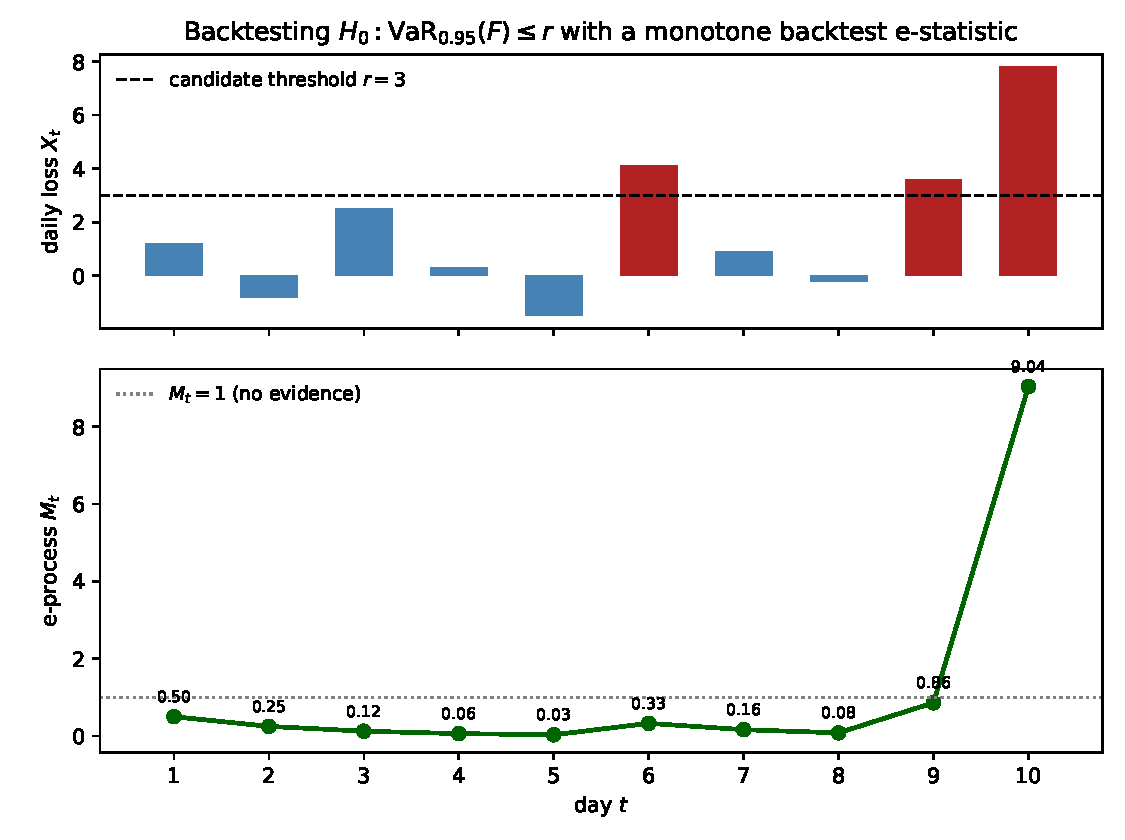
\includegraphics[width=0.72\textwidth]{fig2_eprocess.pdf}
\end{center}
\vspace{-2mm}
{\footnotesize Top: the 10 daily losses, with exceedances of the candidate threshold $r=3$ in red. Bottom: the resulting e-process $M_t = \prod_{s\le t}(0.5+0.5E_s)$ testing $H_0:\mathrm{VaR}_{0.95}(F)\le 3$. Each exceedance multiplies $M_t$ by $10.5$; each non-exceedance multiplies it by $0.5$. The process ends at $M_{10}\approx 9.04$, evidence against $H_0$.}

\end{frame}

% ---------------------------------------------------------------------------
\begin{frame}[fragile]{Python: the full VaR-backtest e-process pipeline}

\begin{lstlisting}
import numpy as np

losses = np.array([1.2, -0.8, 2.5, 0.3, -1.5, 4.1, 0.9, -0.2, 3.6, 7.8])
beta, r, lam = 0.95, 3.0, 0.5

def e_quantile(x, r, beta):
    """Monotone backtest e-statistic for VaR_beta (Example 16.9)."""
    return (1.0 / (1 - beta)) * (x > r)

E = e_quantile(losses, r, beta)                 # one e-variable per day
factors = (1 - lam) + lam * E                   # fractional bet, Eq. (16.15)
M = np.cumprod(factors)                         # the e-process M_t

for t, (x, e_t, m_t) in enumerate(zip(losses, E, M), start=1):
    print(f"day {t:2d}: loss={x:5.2f}  E_t={e_t:5.1f}  M_t={m_t:8.4f}")

print(f"\nFinal e-process M_10 = {M[-1]:.4f}")
print(f"Implied anytime-valid p-value bound: 1/M_10 = {1 / M[-1]:.4f}")
print(f"Exceedance rate observed: {np.mean(losses > r):.0%}  (expected under H0: <= 5%)")
\end{lstlisting}

\end{frame}

% ==========================================================================
\section{Summary}

\begin{frame}{Chapter summary}

\begin{itemize}
\item \textbf{16.1} Risk measures $\mathcal R(X)$/$\rho(F)$ generalize statistical functions like the mean. $\mathrm{VaR}_\beta$ is a quantile; $\mathrm{ES}_\beta$ is the tail-averaged quantile, $\mathrm{ES}_\beta \ge \mathrm{VaR}_\beta$ always. \emph{Coherent} risk measures satisfy monotonicity, cash invariance, subadditivity, and positive homogeneity; $\mathrm{ES}_\beta$ is coherent, $\mathrm{VaR}_\beta$ is not (fails subadditivity/diversification).
\item \textbf{16.2} An e-variable constraint $\EE^{\PP}[E]\le1\ \forall \PP\in\mathcal P$ is exactly a coherent-risk-measure constraint $\mathcal R(E)\le1$ for the super-expectation $\mathcal R(X)=\sup_{\PP\in\mathcal P}\EE^{\PP}[X]$ (Theorem 16.3, Corollary 16.4). $\mathrm{ES}_\beta$ itself has this form, with $\mathcal P$ = measures with likelihood ratio (against a reference) bounded by $1/(1-\beta)$.
\item \textbf{16.3} To test whether a reported risk forecast $r_t$ is honest, build a (monotone) \emph{backtest e-statistic} $e(x,r)$ -- guaranteed power whenever the true risk exceeds $r$ -- and combine sequentially into an e-process $M_t=\prod_s((1-\lambda_s)+\lambda_s E_s)$. Explicit examples exist for the mean, variance, quantiles (VaR), general expected losses, and the Bayes pair $(\mathrm{ES}_\beta,\mathrm{VaR}_\beta)$ (Theorem 16.11).
\end{itemize}

\end{frame}

% ---------------------------------------------------------------------------
\begin{frame}{Bibliographical note}

\begin{itemize}
\item Coherent risk measures were introduced by Artzner et al.\ (1999); the representation in the form of Theorem 16.3 is due to Delbaen (2002), with the law-invariant, continuity-free version by Jouini et al.\ (2006) and Delbaen (2012). Coherent risk measures as pricing formulas: Wang (2000). A broader treatment of risk measures and incomplete-market pricing: F\"ollmer and Schied (2016); risk measures in risk management/regulation: McNeil et al.\ (2015).
\item Formulas (16.1)--(16.2) are due to Rockafellar and Uryasev (2002, Thm.\ 10); the dual representation (16.6), see McNeil et al.\ (2015, Thm.\ 8.14); seven pedagogical proofs of ES subadditivity: Embrechts and Wang (2015).
\item Super-expectations have a long history: axiomatized by Huber (1981, Ch.\ 10) in robust statistics; also central to decision theory under ambiguity (Schmeidler 1989; Gilboa and Schmeidler 1989), imprecise probabilities (Walley 1991), nonlinear expectations (Peng 2019), and game-theoretic probability (Shafer and Vovk 2001, 2019).
\item Section 16.3 is largely based on Wang et al.\ (2025), who show most backtest e-statistics here are essentially the only possible choices, and study financial backtesting applications. Forecast comparison via e-processes: Henzi and Ziegel (2022). Sequential quantile testing/estimation: Howard and Ramdas (2022). Bayes pairs: Embrechts et al.\ (2021). The ES/VaR backtest e-statistic (Theorem 16.11) connects to the joint elicitability of ES and VaR (Fissler and Ziegel, 2016). Mean/variance e-processes: Fan et al.\ (2025).
\end{itemize}

\end{frame}

\end{document}
